\part{Chapitre 1}
 \section{Définitions}
 \subsection{Le Volt}
 Le \textbf{Volt} est définit de telle manière qu'une charge d'un \textbf{Coulomb} accéléré sous une tension d'unV acquiert une énergie de un \textbf{Joule}.\\
 \begin{equation}
	 U = \frac{W}{Q}
 \end{equation}

 \begin{equation}
	 [V] = \frac{[J]}{[Q]}
 \end{equation}
 Avec:
 \begin{itemize}
	 \item \textbf{U}: La tension en \textbf{Volt} (\textit{V})
	 \item \textbf{W}: L'énergie en \textbf{Joule} (\textit{J})
	 \item \textbf{Q}: La charge électrique en \textbf{Coulomb} (\textit{C})
 \end{itemize}

 \subsection{L'ampère}
 L'\textbf{ampère} est l'intensité de courant qui existe quand une charge d'un \textbf{Coulomb} franchit la subsection transversale d'un conducteur en une \textbf{seconde}.\\
 \begin{equation}
	 I = \frac{Q}{t}
 \end{equation}
 \begin{equation}
	 [A] = \frac{[C]}{[s]}
 \end{equation}

 \begin{itemize}
	 \item \textbf{I}: L'intensité du courant en \textbf{Ampère} (\textit{A})
	 \item \textbf{Q}: La charge électrique en \textbf{Coulomb} (\textit{C})
	 \item \textbf{t}: Le temps en \textbf{seconde} (\textit{s})
 \end{itemize}

 \subsection{Coulomb}
 Un \textbf{Coulombs} est définit comme la charge transportée par \textbf{$6.25*10^{18}$} électrons.

 \section{Lois et formules importantes}

 \subsection{Loi de Pouillet}

 \begin{equation}
	 R=\frac{\rho.l}{S}
 \end{equation}

 \begin{equation}
	 [\Omega] = \frac{[\Omega.m].[m]}{[m^2]}
 \end{equation}

 \begin{itemize}
	 \item \textbf{R}: La résistance du fil en \textbf{Ohm} (\textit{A})
	 \item \textbf{$\rho$}: La résistivité de matériau en \textbf{Ohm mètre} (\textit{$\Omega$.m})
	 \item \textbf{l}: La longeur du fil en \textbf{mètre} (\textit{m})
	 \item \textbf{S}: La subsection de fil en \textbf{mètre carré} (\textit{m\textsuperscript{2}})
 \end{itemize}
 Cette loi est valable à 0°C.

 \subsection{Loi de Mathiessen}

 \begin{equation}
	 R_{T}=R_{0}.(1+\alpha.T)
 \end{equation}

 \begin{itemize}
	 \item \textbf{R\textsubscript{T}}: La résistance du fil à la température T en \textbf{Ohm} (\textit{A})
	 \item \textbf{R\textsubscript{0}}: La résistance du fil à 0°C en \textbf{Ohm} (\textit{A})
	 \item \textbf{$\alpha$}: Le coefficient de température en (\textit{°C\textsuperscript{-1}})
	 \item \textbf{T}: La température en \textbf{degré Celcius} (\textit{°C})
 \end{itemize}
 Cette lois s'applique aussi pour les résistivités.

 \subsection{Loi d'Ohm}

 \begin{equation}
	 R=\frac{U}{I}
 \end{equation}

 \begin{equation}
	 [\Omega]=\frac{[\Omega]}{[A]}
 \end{equation}

 \begin{itemize}
	 \item \textbf{R}: La résistance en \textbf{Ohm} (\textit{A})
	 \item \textbf{U}: La tension en \textbf{Volt} (\textit{V})
	 \item \textbf{I}: L'intensité du courant en \textbf{Ampère} (\textit{A})
 \end{itemize}

 \subsection{La puissance}

 \begin{equation}
	 P=U.I
 \end{equation}

 \begin{equation}
	 [W]=[V].[A]
 \end{equation}

 \begin{itemize}
	 \item \textbf{P}: La puissance en \textbf{Watt} (\textit{W})
	 \item \textbf{U}: La tension en \textbf{Volt} (\textit{V})
	 \item \textbf{I}: L'intensité du courant en \textbf{Ampère} (\textit{A})
 \end{itemize}

 \subsection{L'effet joule}

 Si le récepteur est purement calorifique:
 \begin{equation}
	 W_{cal} = R.I^2.t
 \end{equation}

 \begin{equation}
	 [J]=[\Omega].{[A]}^2.[s]
 \end{equation}

 \begin{itemize}
	 \item \textbf{W}: Le travaille en \textbf{Joule} (\textit{J})
	 \item \textbf{R}: La résistance en \textbf{Ohm} (\textit{A})
	 \item \textbf{I}: L'intensité du courant en \textbf{Ampère} (\textit{A})
	 \item \textbf{t}: Le temps en \textbf{seconde} (\textit{s})
 \end{itemize}

 \subsection{La loi des noeuds}

 \begin{equation}
	 \sum I_{entrants} = \sum I_{sortants}
 \end{equation}

 \subsection{La loi des mailles}

 \begin{equation}
	 \sum U_{maille} = \sum U_{\text{dans un sens}}
 \end{equation}

 \subsection{Récepteurs mis en série}
 \subsubsection{Courant}

 \hyprref[Vidéo exemple]{https://www.youtube.com/watch?v=CENFfGLFPrE}

 \begin{equation}
	 I_{AB} = I_{BC} = I_{tot}
 \end{equation}

 \subsubsection{Différence de potentiel}

 \begin{equation}
	 U_{AB} + U_{BC} = U_{tot}
 \end{equation}

 \subsubsection{Résistances}

 \begin{equation}
	 R_{eq} = \sum R_{série}
 \end{equation}

 \subsection{Récepteurs mis en parallèle}
 \subsubsection{Courant}

 \begin{equation}
	 I_{AB} + I_{BC} = I_{tot}
 \end{equation}
 C'est la loi des noeuds

 \subsubsection{Différence de potentiel}

 \begin{equation}
	 U_{AB} = U_{BC} = U_{tot}
 \end{equation}

 \subsubsection{Résistances}

 \begin{equation}
	 \frac{1}{R_{eq}} = \sum \frac{1}{R_{parallèle}}
 \end{equation}
 \begin{equation}
	 R_{eq} = \frac{\prod R_{parallèle}}{\sum R_{parallèle}}
 \end{equation}

 \subsection{Théorème de Kennelly}

\begin{figure}[h]
	 \centering
	 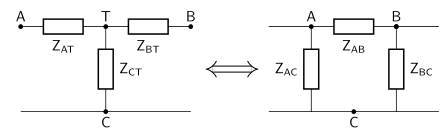
\includegraphics[scale = 0.5]{kennelly}
	 \caption{Transformation d'une étoile par le théorème de Kennelly}
 \end{figure}

 \begin{equation}
	 R_{AT} = \frac{R_{AB}.R_{AC}}{R_{AB} + R_{AC}+R_{BC}}
 \end{equation}

 \begin{equation}
	 R_{BT} = \frac{R_{BA}.R_{BC}}{R_{AB} + R_{AC}+R_{BC}}
 \end{equation}

 \begin{equation}
	 R_{CT} = \frac{R_{CA}.R_{CB}}{R_{AB} + R_{AC}+R_{BC}}
 \end{equation}
